\documentclass[conf]{new-aiaa}

\usepackage{subcaption}
\usepackage{enumitem}

\title{Optimal Racing Line and Energy Management for Electric Vehicles under Uncertain Grip}

\author{
  Erwin Poussi
  \ and
  Matthieu Hautsch\\
  {\normalsize\itshape Stanford University, Stanford, CA 94305}
}

\begin{document}

\maketitle

\begin{abstract}
Autonomous racing pushes the limits of control and optimization, requiring vehicles to navigate circuits at the edge of their physical capabilities. For electric vehicles, performance is further constrained by battery energy, making the racing line problem inherently multiobjective. We formulate the joint optimization of racing line and speed profile on closed circuits and solve it through three stages. First, we compute the time-optimal trajectory using a custom Sequential Convex Programming (SCP) algorithm with a hand-coded Simplex solver, validated against scipy's Sequential Least Squares Programming (SLSQP). Second, we trace the Pareto front between lap time and energy consumption via a weighted-sum formulation. Third, we extend the optimization to uncertain tire grip using Sample Average Approximation (SAA). On our test circuit, both solvers converge to a 27\,s optimal lap time, and the robust Pareto front under grip uncertainty is shifted toward safer, slower operating points.
\end{abstract}

\section{Introduction}

Finding the fastest path around a race track is a classical problem in vehicle dynamics and motorsport engineering~\cite{Xiong2010, Heilmeier2020}. The trajectory followed by a vehicle directly determines the curvature encountered along the track and therefore the maximum speed that can be maintained through each corner. By exploiting the full width of the track, drivers reduce curvature and increase cornering speed, leading to significant reductions in lap time.

For electric vehicles, racing line optimization becomes a multi-objective problem. In addition to minimizing lap time, the vehicle must manage a finite energy budget. Aggressive acceleration and high cornering speeds improve performance but increase energy consumption, while conservative driving strategies preserve battery charge at the cost of slower lap times. This tradeoff is particularly relevant in modern electric racing series such as Formula E~\cite{Sciarretta2007} and in autonomous racing applications.

This project investigates the computation of optimal racing trajectories for electric vehicles under both deterministic and uncertain operating conditions. We formulate the problem as a nonlinear optimization over the racing line and speed profile and study the tradeoff between lap time and energy consumption. We further analyze the impact of uncertain tire grip through a robust optimization framework.

Our approach is organized into three stages: (1)~time-optimal racing line optimization using a kinematic vehicle model and Sequential Convex Programming (SCP), (2)~multi-objective optimization of lap time and energy consumption through Pareto front analysis, and (3)~robust optimization under uncertain tire-road friction using Sample Average Approximation (SAA). The optimized trajectories are subsequently tracked using a dynamic bicycle model and a Time-Varying Linear Quadratic Regulator (TV-LQR) to evaluate their feasibility in closed-loop simulation.

\section{Problem Formulation}

\subsection{Optimization Overview}

The objective is to jointly optimize the geometric racing line and the corresponding speed profile around a closed circuit. We first compute the minimum-time trajectory considering only kinematic constraints, then extend the formulation to include battery energy consumption and generate a Pareto front, and finally account for uncertainty in tire grip to compute robust trajectories that remain feasible under adverse friction conditions. Figure~\ref{fig:decision_vars} illustrates the track parameterization and the optimization variables.

\subsection{Decision Variables}

The racing line is parameterized using lateral offsets $\boldsymbol{\alpha} = (\alpha_1, \dots, \alpha_n)$ measured from the track centerline. At station $i$, the vehicle position is $\mathbf{p}_i = \mathbf{c}_i + \alpha_i \hat{\mathbf{n}}_i$, where $\mathbf{c}_i$ denotes the centerline position and $\hat{\mathbf{n}}_i$ the outward normal direction. The constraint $|\alpha_i| \leq w_i$ keeps the path within the track of half-width $w_i$. The speed profile is $\mathbf{v} = (v_1, \dots, v_n)$, and the complete optimization vector is $\mathbf{x} = (\boldsymbol{\alpha}, \mathbf{v}) \in \mathbb{R}^{2n}$.

\begin{figure}[h]
  \centering
  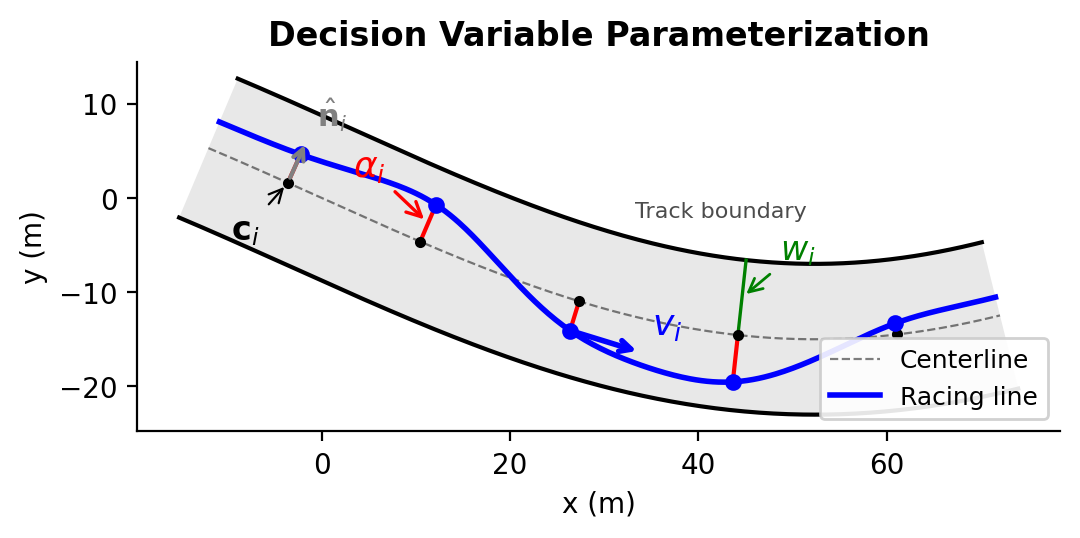
\includegraphics[width=0.5\linewidth]{../figures/decision_variables.png}
  \caption{Track parameterization and optimization variables. The lateral offset $\alpha_i$ displaces each path point from the centerline $\mathbf{c}_i$ along the normal $\hat{\mathbf{n}}_i$. The speed $v_i$ is along the tangent; $w_i$ bounds the feasible region.}
  \label{fig:decision_vars}
\end{figure}

\subsection{Vehicle and Track Dynamics}

The optimization uses a kinematic point-mass model that captures the dominant physical limitations. At each station, the centripetal acceleration required to follow the curved path must not exceed the available tire friction:
\begin{equation}\label{eq:cornering}
  v_i^2 \, |\kappa_i(\boldsymbol{\alpha})| \leq 0.85\,\mu \, g
\end{equation}
where 0.85 is a safety margin. Between consecutive stations, longitudinal dynamics are bounded by the vehicle's acceleration and braking capabilities:
\begin{equation}\label{eq:accel}
  v_{i+1}^2 \leq v_i^2 + 2\,a_{\text{lon}}\,\Delta s_i, \quad
  v_i^2 \leq v_{i+1}^2 + 2\,a_{\text{brk}}\,\Delta s_i
\end{equation}
where $\Delta s_i = \|\mathbf{p}_{i+1} - \mathbf{p}_i\|$ is the segment arc length.

\subsection{Lap Time Objective}

The total lap time is
\begin{equation}\label{eq:laptime}
  T(\boldsymbol{\alpha}, \mathbf{v}) = \sum_{i=1}^{n} \frac{\Delta s_i(\boldsymbol{\alpha})}{v_i}
\end{equation}
This objective is nonlinear in both $\boldsymbol{\alpha}$ (through $\Delta s_i$) and $\mathbf{v}$.

\subsection{Energy Consumption Model}

At each segment, the traction force accounts for inertial, aerodynamic, and rolling resistance contributions: $F_i = m\,a_i + \tfrac{1}{2}\rho C_d A\,v_i^2 + C_r m g$. The mechanical power is $P_i = F_i \cdot v_i$. Depending on the sign of $P_i$, the electrical energy integrates $P_i / \eta$ during drive phases or recovers $|P_i| \cdot \eta_{\text{regen}}$ during braking. Summing over all segments yields the total energy expenditure $E(\boldsymbol{\alpha}, \mathbf{v})$. All notation and vehicle parameters are gathered in Appendix~\ref{app:notation}.

\section{Time-Optimal Racing Line Using SCP}

The first stage finds the time-optimal racing line and speed profile under constraints~\eqref{eq:cornering}--\eqref{eq:accel}. Since both the objective and constraints are nonlinear, we use Sequential Convex Programming (SCP) following the trust-region approach in~\cite{Kochenderfer2019}. At each iteration, we linearize all nonlinear constraints around the current iterate and solve the resulting linear program (LP):
\begin{equation}\label{eq:lp}
  \min_{\Delta\mathbf{x}} \; \mathbf{c}^\top \Delta\mathbf{x} \quad \text{s.t.} \quad \mathbf{A}\,\Delta\mathbf{x} \leq \mathbf{b}, \quad \boldsymbol{\ell} \leq \Delta\mathbf{x} \leq \mathbf{u}
\end{equation}
where $\mathbf{c}$ is the linearized objective gradient. The constraint matrix $\mathbf{A} \in \mathbb{R}^{3n \times 2n}$ stacks the Jacobians of the cornering, acceleration, and braking constraints, and $\mathbf{b}$ contains the corresponding right-hand sides evaluated at the current iterate (see Appendix~\ref{app:scp} for full expressions). The bounds $(\boldsymbol{\ell}, \mathbf{u})$ enforce both the trust region $|\Delta\alpha_i| \leq \rho$ and the variable limits. We solve this LP with a two-phase Simplex algorithm~\cite{Kochenderfer2019} implemented from scratch. The curvature Jacobian $\partial\kappa_i / \partial\alpha_j$ is computed with JAX automatic differentiation.

The trust region radius $\rho$ adapts at each iteration: halved when the step causes large constraint violations, grown by a factor of 1.2 when the step improves the objective. To validate the SCP solution, we solve the same problem with scipy's SLSQP. SCP converges from 34.6\,s to 26.9\,s in 15 iterations, while SLSQP reaches 26.8\,s in 94 iterations, confirming that both solvers find the global optimum.

\section{Time-Energy Pareto Optimization}

The second stage addresses the tradeoff between lap time and energy consumption. For an electric vehicle that must complete multiple laps, aggressive time-optimal trajectories can discharge the battery rapidly and may not represent the best overall race strategy. To explore this tradeoff, we use the weighted-sum method~\cite{Kochenderfer2019}:
\begin{equation}\label{eq:pareto}
  \min_{\boldsymbol{\alpha}, \mathbf{v}} \; (1-w) \frac{T}{T_{\text{ref}}} + w \frac{E}{E_{\text{ref}}}
\end{equation}
where $T_{\text{ref}}$ and $E_{\text{ref}}$ are reference values from the time-optimal solution. Sweeping $w \in [0, 0.95]$ traces the Pareto front.

When we attempted to compute the Pareto front with SCP, the algorithm failed for most $w > 0$. As the energy weight increases, the optimal speed profile shifts far from the warm start. The linearized constraints become poor approximations, causing violations that trigger trust region shrinkage until convergence stalls. We therefore use scipy's SLSQP for the Pareto computation. The resulting Pareto front is shown in Figure~\ref{fig:pareto}.

\section{Robust Optimization under Uncertain Grip}

In practice, tire grip varies along the track due to wet patches, rubber deposits, or temperature gradients. We model this by treating the friction coefficient as a per-station random variable: $\mu_i \sim \mathcal{N}(1.0, \sigma_\mu^2)$, clipped to $[0.3, 1.5]$, with $\sigma_\mu = 0.1$.

We handle the stochastic constraints with Sample Average Approximation (SAA)~\cite{Kochenderfer2019}. We draw $N = 20$ scenarios, each providing a grip vector $\boldsymbol{\mu}^{(k)}$. Since the cornering constraint is monotone in $\mu$, it suffices to enforce the worst-case grip at each station:
\begin{equation}\label{eq:saa}
  v_i^2 \, |\kappa_i| \leq \mu_i^{\text{worst}} \cdot g \cdot 0.85, \quad \mu_i^{\text{worst}} = \min_{k} \mu_i^{(k)}
\end{equation}
This reduces $N \times n$ scenario constraints to $n$ deterministic constraints with modified grip, making the robust problem no more expensive than the nominal one.

\section{Dynamic Trajectory Tracking}

The kinematic optimization produces a racing line and speed profile, but these are not directly executable by a vehicle with tire slip and yaw dynamics. To bridge this gap, we formulate the trajectory tracking as a finite-horizon optimal control problem (full dynamics in Appendix~\ref{app:dynamics}).

Given a reference trajectory $(\bar{\mathbf{s}}_k, \bar{\mathbf{u}}_k)_{k=0}^{N}$, we seek the control sequence that minimizes tracking error:
\begin{equation}\label{eq:lqr_cost}
  \min_{\mathbf{u}_{0:N-1}} \sum_{k=0}^{N-1} \bigl[(\mathbf{s}_k - \bar{\mathbf{s}}_k)^\top Q\, (\mathbf{s}_k - \bar{\mathbf{s}}_k) + (\mathbf{u}_k - \bar{\mathbf{u}}_k)^\top R\, (\mathbf{u}_k - \bar{\mathbf{u}}_k)\bigr]
\end{equation}
subject to the bicycle dynamics $\mathbf{s}_{k+1} = f(\mathbf{s}_k, \mathbf{u}_k)$, where $\mathbf{s} = [x, y, \psi, v_x, v_y, \omega]^\top$ and $\mathbf{u} = [\delta, F_{\text{drive}}]^\top$.

We solve this in two phases. First, a Stanley lateral controller tracks the kinematic racing line to generate a dynamically feasible reference $(\bar{\mathbf{s}}_k, \bar{\mathbf{u}}_k)$ consistent with the bicycle model. Second, we linearize the dynamics around each reference point via finite differences to obtain $A_k = \partial f / \partial \mathbf{s}$ and $B_k = \partial f / \partial \mathbf{u}$, then solve the discrete Riccati equation backward to compute the TV-LQR gains $K_k$ (see Appendix~\ref{app:tvlqr}). Online, the control law is
\begin{equation}
  \mathbf{u}_k = \bar{\mathbf{u}}_k + K_k (\mathbf{s}_k - \bar{\mathbf{s}}_k)
\end{equation}
with spatial indexing to handle timing mismatches between the reference and the actual vehicle state.

\section{Results}

\subsection{SCP vs SLSQP Convergence}

Figure~\ref{fig:convergence} shows the convergence of both solvers on our test circuit (40 stations, 903\,m). SCP converges from 34.6\,s to 26.9\,s in 15 iterations, while SLSQP requires 94 iterations to reach 26.8\,s, confirming that both solvers reach the global optimum. As a baseline, following the track centerline with the same velocity profile computation yields a lap time of 40.3\,s. The optimized racing line thus reduces lap time by 33\%, demonstrating the benefit of exploiting the full track width.

\subsection{Time-Energy Pareto Front}

Figure~\ref{fig:pareto} presents the nominal and robust Pareto fronts. At $w = 0$, the nominal optimum matches the SCP result. As $w$ increases, the optimizer trades lap time for energy savings, reaching $\sim$44\,s at $w = 0.95$ with near-zero net energy. The robust front is shifted to longer lap times: at $w = 0$, the robust optimum is $\sim$30\,s versus 27\,s, a 3\,s penalty that quantifies the cost of robustness. However, this penalty shrinks as energy becomes more important in the objective, since energy-efficient trajectories are inherently smoother with lower cornering loads, reducing the sensitivity to grip uncertainty.

\begin{figure}[h!]
  \centering
  \begin{subfigure}[t]{0.48\linewidth}
    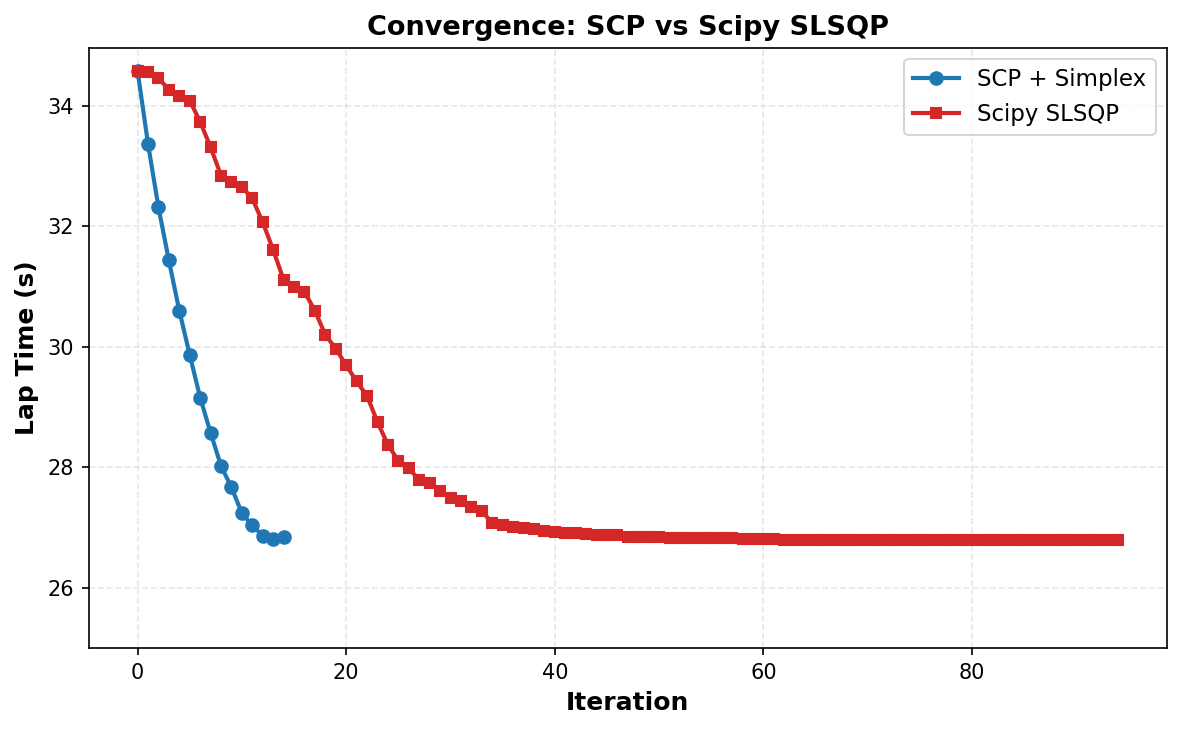
\includegraphics[width=\linewidth]{../figures/convergence_scp_vs_scipy.png}
    \caption{Convergence of SCP+Simplex vs SLSQP.}
    \label{fig:convergence}
  \end{subfigure}
  \hfill
  \begin{subfigure}[t]{0.48\linewidth}
    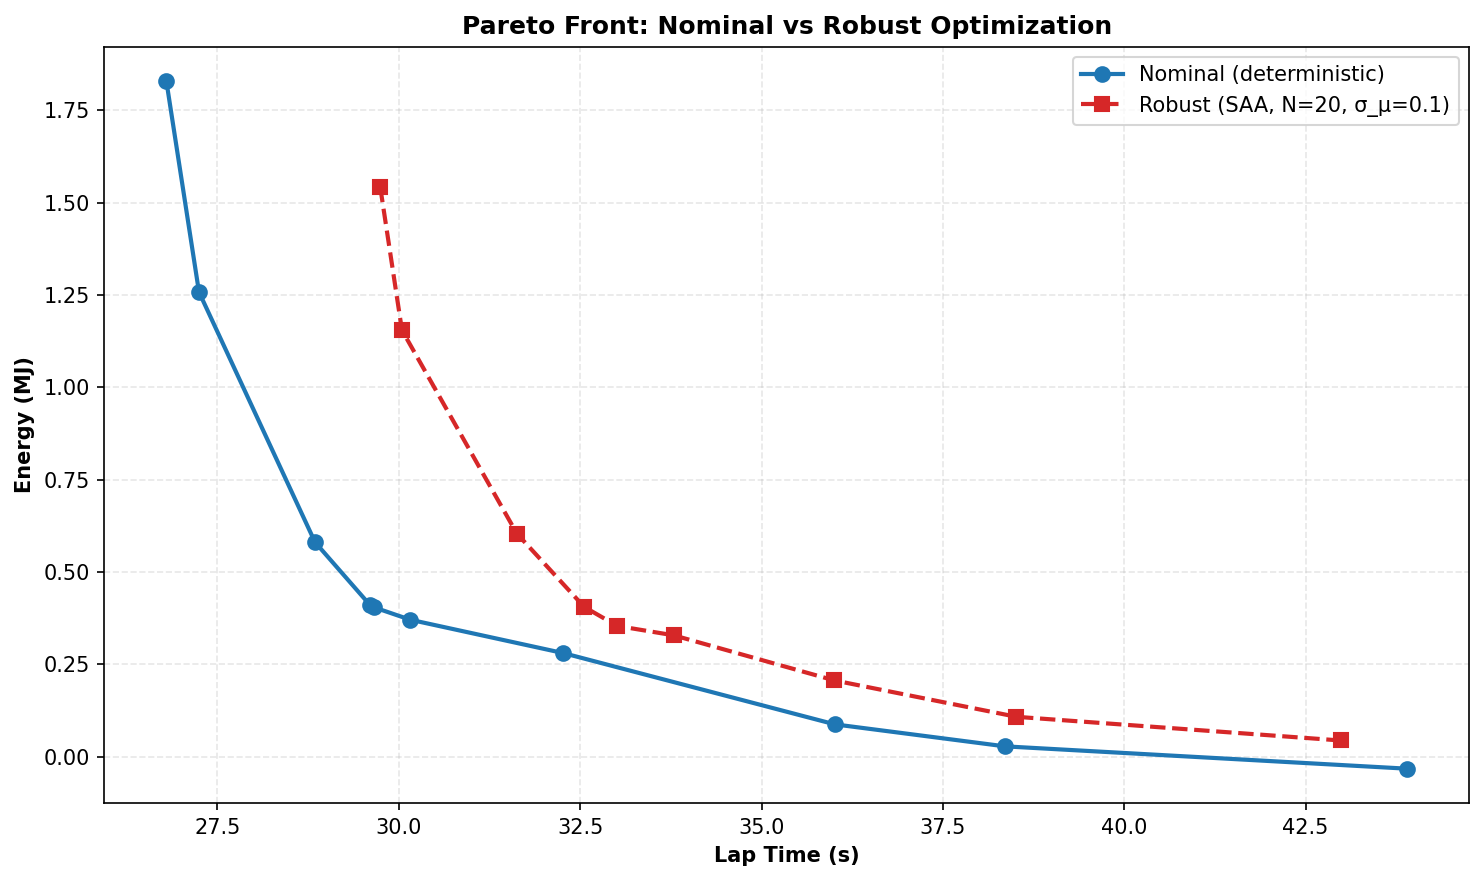
\includegraphics[width=\linewidth]{../figures/pareto_nominal_vs_robust.png}
    \caption{Nominal and robust Pareto fronts.}
    \label{fig:pareto}
  \end{subfigure}
  \caption{(a) Both solvers reach $\sim$27\,s, but SCP converges in fewer iterations. (b) The robust front is shifted to longer lap times due to worst-case grip constraints.}
\end{figure}

\subsection{Nominal vs Robust Trajectories}

Figure~\ref{fig:nom_vs_rob} compares the nominal and robust racing lines and speed profiles. The geometric racing lines are nearly identical since curvature reduction is grip-independent. The robust speed profile, however, is consistently lower, reflecting the conservatism of the worst-case SAA constraint. Yet the profile retains the same shape and variations as the nominal one: the vehicle still accelerates on straights and brakes into corners, only at reduced magnitudes.

\begin{figure}[h!]
  \centering
  \begin{subfigure}[t]{0.48\linewidth}
    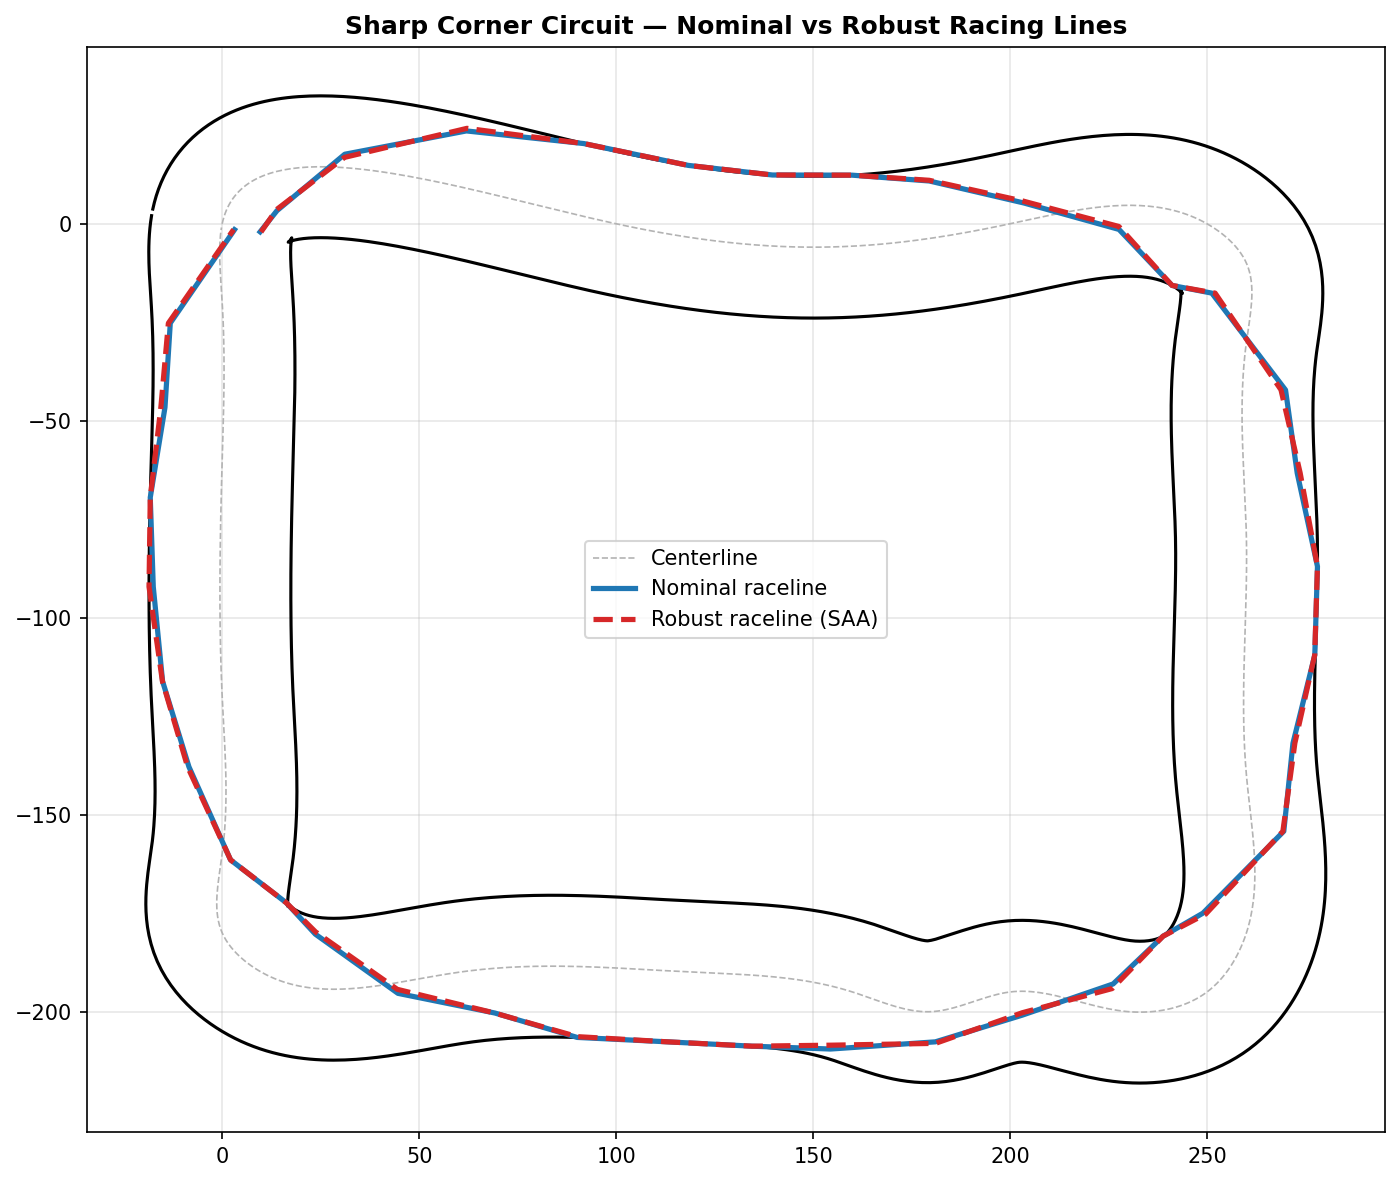
\includegraphics[width=\linewidth]{../figures/raceline_nom_vs_robust.png}
    \caption{Racing lines on the track.}
  \end{subfigure}
  \hfill
  \begin{subfigure}[t]{0.48\linewidth}
    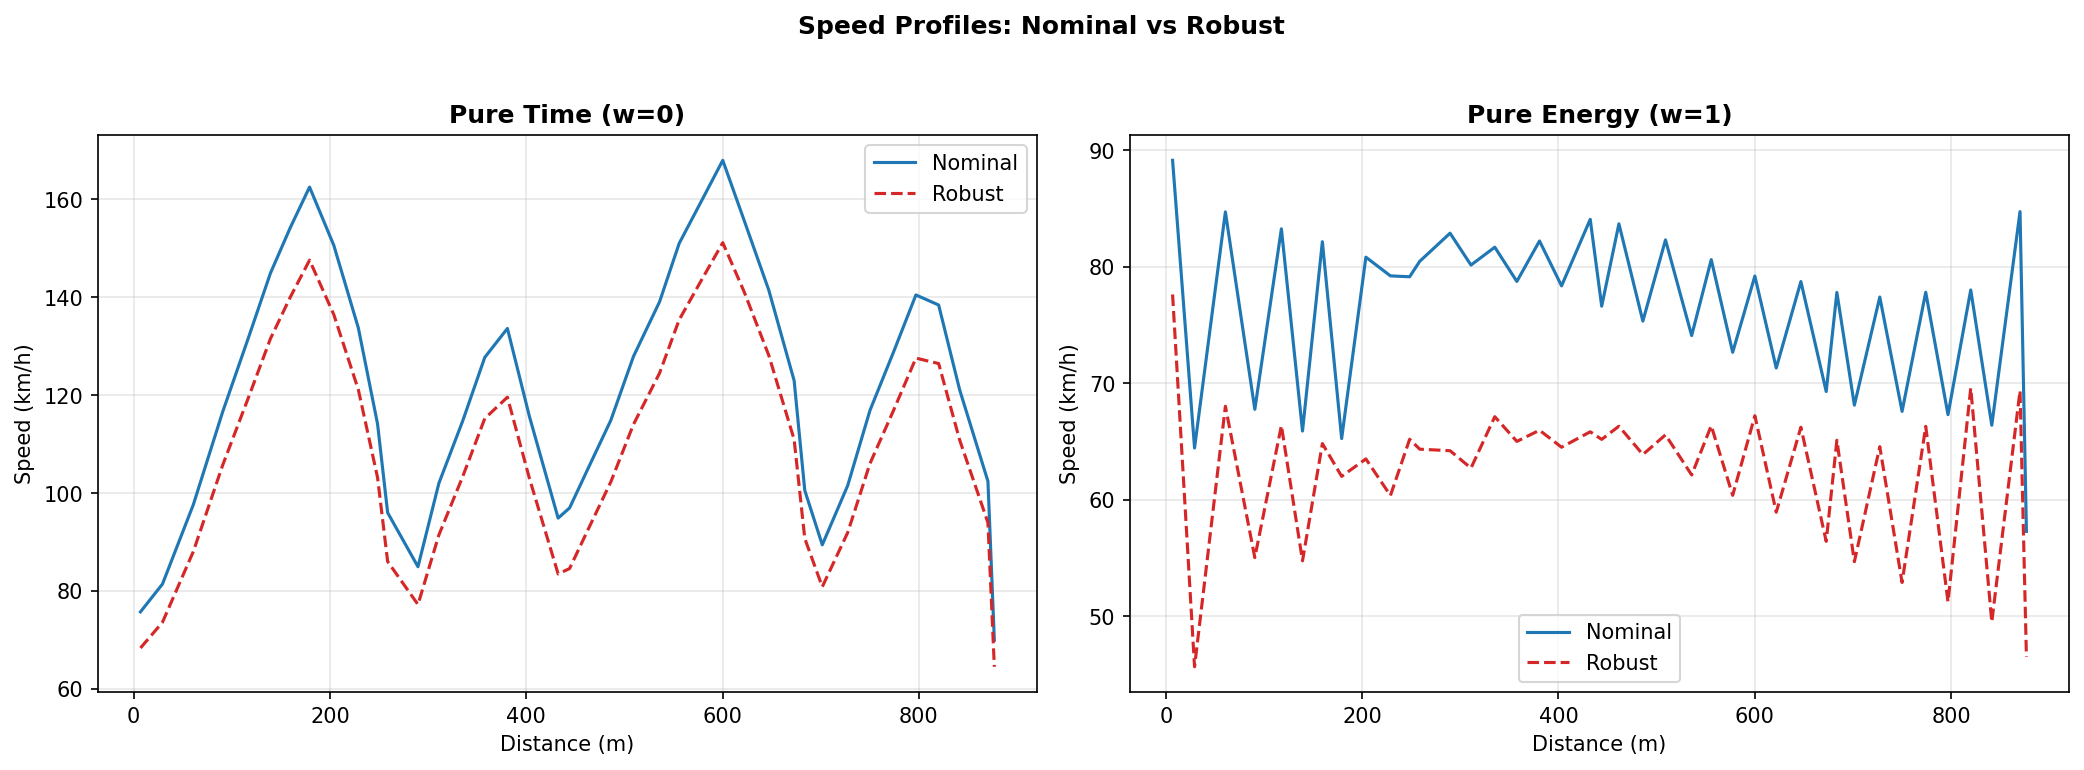
\includegraphics[width=\linewidth]{../figures/speed_profiles_nom_vs_robust.png}
    \caption{Speed profiles along the track.}
  \end{subfigure}
  \caption{Nominal vs robust trajectories. The geometric paths are similar, but the robust profile maintains lower speeds throughout.}
  \label{fig:nom_vs_rob}
\end{figure}

\section{Conclusion}

This work presented an optimization framework for electric vehicle racing that combines trajectory optimization, energy management, and robustness to uncertain tire grip. The SCP formulation efficiently solved the minimum-time problem (15 iterations vs 94 for SLSQP) while reaching the same optimum. Multi-objective optimization revealed that small increases in lap time (27\,s to 32\,s) yield large energy savings. The robust SAA formulation added a 3\,s penalty at the time-optimal point, with the gap narrowing for energy-efficient trajectories.

A key limitation is the gap between kinematic optimization and dynamic feasibility. The kinematic model overpredicts cornering speed because it ignores tire slip and yaw inertia. Closing this gap would require incorporating vehicle dynamics directly into the optimization. Future work will also focus on extending the uncertainty model and investigating chance-constrained formulations that reduce conservatism while maintaining robustness.

\section*{Contributions}

Erwin Poussi developed the simulator, the SCP algorithm with Simplex and the scipy SLSQP pipeline, the iLQR trajectory tracking controller, the race simulation engine, and the stochastic optimization formulation. Matthieu Hautsch implemented the Pareto front analysis and the energy consumption model.

\bibliography{references}

\newpage
\begin{center}
  {\Large\bfseries Supplementary Material}
\end{center}
\vspace{1em}

\appendix

\section{Notation and Vehicle Parameters}\label{app:notation}

\begin{table}[h!]
\centering
\small
\begin{tabular}{lll}
\toprule
Symbol & Value & Description \\
\midrule
$m$ & 1600\,kg & Vehicle mass \\
$L$ & 2.9\,m & Wheelbase \\
$l_f,\, l_r$ & 1.4,\, 1.5\,m & CG to front/rear axle \\
$I_z$ & 2500\,kg\,m$^2$ & Yaw moment of inertia \\
$\mu$ & 1.0 & Tire-road friction coefficient \\
$C_f,\, C_r$ & 80\,000,\, 90\,000\,N/rad & Cornering stiffness (front/rear) \\
$C_d$ & 0.30 & Aerodynamic drag coefficient \\
$A$ & 1.5\,m$^2$ & Frontal area \\
$\rho$ & 1.225\,kg/m$^3$ & Air density \\
$C_r$ & 0.012 & Rolling resistance coefficient \\
$P_{\max}$ & 250\,kW & Maximum motor power \\
$F_{\text{drive,max}}$ & 8\,000\,N & Maximum traction force \\
$F_{\text{brake,max}}$ & 12\,000\,N & Maximum braking force \\
$\eta$ & 0.92 & Motor efficiency \\
$\eta_{\text{regen}}$ & 0.65 & Regenerative braking efficiency \\
$v_{\max}$ & --- & Speed limit (power-limited) \\
$g$ & 9.81\,m/s$^2$ & Gravitational acceleration \\
\bottomrule
\end{tabular}
\caption{Vehicle parameters used in the optimization and simulation.}
\end{table}

\section{Bicycle Model Dynamics}\label{app:dynamics}

The dynamic bicycle model used for trajectory tracking has state $\mathbf{s} = [x, y, \psi, v_x, v_y, \omega]^\top$ and control $\mathbf{u} = [\delta, F_{\text{drive}}]^\top$. The continuous-time equations of motion are:
\begin{align}
  \dot{x} &= v_x \cos\psi - v_y \sin\psi \\
  \dot{y} &= v_x \sin\psi + v_y \cos\psi \\
  \dot{\psi} &= \omega \\
  \dot{v}_x &= \frac{1}{m}\bigl(F_{\text{drive}} - F_{\text{drag}} - F_{\text{roll}} + m\,v_y\,\omega - F_{yf}\sin\delta\bigr) \\
  \dot{v}_y &= \frac{1}{m}\bigl(F_{yf}\cos\delta + F_{yr} - m\,v_x\,\omega\bigr) \\
  \dot{\omega} &= \frac{1}{I_z}\bigl(l_f\,F_{yf}\cos\delta - l_r\,F_{yr}\bigr)
\end{align}
where the lateral tire forces use a linear slip angle model with saturation:
\begin{align}
  \alpha_f &= \delta - \arctan\!\frac{v_y + l_f\,\omega}{v_x}, \quad
  \alpha_r = -\arctan\!\frac{v_y - l_r\,\omega}{v_x} \\
  F_{yf} &= \text{clip}(C_f\,\alpha_f,\; -F_{\text{lim}},\; F_{\text{lim}}), \quad
  F_{yr} = \text{clip}(C_r\,\alpha_r,\; -F_{\text{lim}},\; F_{\text{lim}})
\end{align}
with $F_{\text{lim}} = \tfrac{1}{2}\mu\,m\,g$. The resistive forces are $F_{\text{drag}} = \tfrac{1}{2}\rho\,C_d\,A\,v_x^2$ and $F_{\text{roll}} = C_r\,m\,g$. The drive force is further limited by power: $F_{\text{drive}} \leq P_{\max}/v_x$ when $F_{\text{drive}} > 0$. These equations are integrated using a fourth-order Runge-Kutta scheme at $\Delta t = 0.02$\,s.

\section{SCP Sub-Problem Construction}\label{app:scp}

At SCP iteration with current iterate $(\boldsymbol{\alpha}, \mathbf{v})$, the LP~\eqref{eq:lp} is constructed as follows. Let $\Delta\mathbf{x} = (\Delta\boldsymbol{\alpha}, \Delta\mathbf{v})$.

\textbf{Objective gradient.} The linearized lap time gradient is:
\begin{equation}
  \mathbf{c} = \begin{bmatrix} \dfrac{\partial \mathbf{ds}}{\partial \boldsymbol{\alpha}}^\top \dfrac{1}{\mathbf{v}} \\[6pt] -\dfrac{\mathbf{ds}}{\mathbf{v}^2} \end{bmatrix}
\end{equation}
where $\mathbf{ds}$ is the vector of segment lengths and the Jacobian $\partial \mathbf{ds}/\partial\boldsymbol{\alpha}$ is computed from the path geometry.

\textbf{Cornering constraints.} Linearizing $v_i^2|\kappa_i| \leq a_{\text{lat}}$ around the current iterate yields rows of $\mathbf{A}$ involving $v_i^2 \cdot \text{sgn}(\kappa_i) \cdot \partial\kappa_i/\partial\alpha_j$ (from JAX autodiff) and $2\,v_i\,|\kappa_i|$.

\textbf{Acceleration/braking constraints.} Similarly linearized from~\eqref{eq:accel}, coupling consecutive speed variables through the segment-length Jacobian.

\section{TV-LQR Gain Computation}\label{app:tvlqr}

Given the reference trajectory $(\bar{\mathbf{s}}_k, \bar{\mathbf{u}}_k)$, we compute the discrete Jacobians $A_k \in \mathbb{R}^{6\times 6}$ and $B_k \in \mathbb{R}^{6\times 2}$ by finite differences of the RK4 integrator. The TV-LQR gains are obtained by solving the discrete Riccati equation backward:
\begin{align}
  K_k &= -(R + B_k^\top P_{k+1} B_k)^{-1} B_k^\top P_{k+1} A_k \label{eq:Kgain}\\
  P_k &= Q + A_k^\top P_{k+1} (A_k + B_k K_k) \label{eq:riccati}
\end{align}
with terminal condition $P_N = Q$. The weight matrices are $Q = \text{diag}(5,\, 5,\, 10,\, 1,\, 0.5,\, 0.5)$ and $R = \text{diag}(10,\, 10^{-5})$, penalizing position and heading errors more heavily than lateral velocity, while keeping steering effort smooth.

\end{document}
